%************************************************
\section{Identifying objects to monitor} % (fold)
\label{sec:sd_identify_objects}
%************************************************
In the assets, right click the ''Scenes/childproof/childproof.j3o'' file and select ''Edit in SceneComposer'' as illustrated in Figure \ref{fig:sd_edit_in_scene_composer}.
\begin{figure}[H]
	\centering
	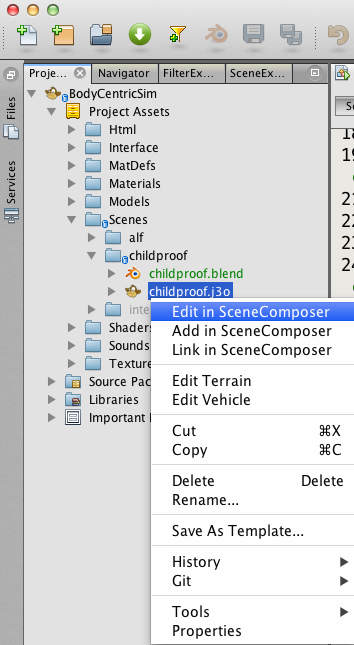
\includegraphics[width=0.5\linewidth]{gfx/Chapter_SD_UserGuide/edit_in_scene_composer}
	\caption{Edit in Scene Composer}
	\label{fig:sd_edit_in_scene_composer}
\end{figure}

To see the environment, you'll have to ''turn on the lights'', as depicted in Figure \ref{fig:sd_light_in_scene_composer}.
\begin{figure}[H]
	\centering
	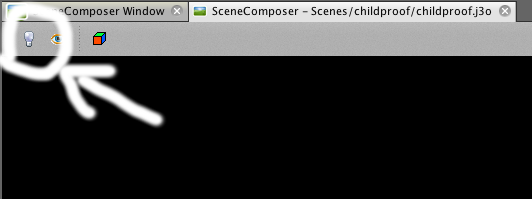
\includegraphics[width=\linewidth]{gfx/Chapter_SD_UserGuide/scenecomposer_light}
	\caption{Turning on the light in Scene Composer}
	\label{fig:sd_light_in_scene_composer}
\end{figure}

Suppose that the objects you want to track in this scenario are the Outlets and all the small objects that might be inserted into them; in this case, the pen on the living room table. These objects are highlighted in the screen-shot from Figure \ref{fig:sd_objects_to_identify}.
\begin{figure}[H]
	\centering
	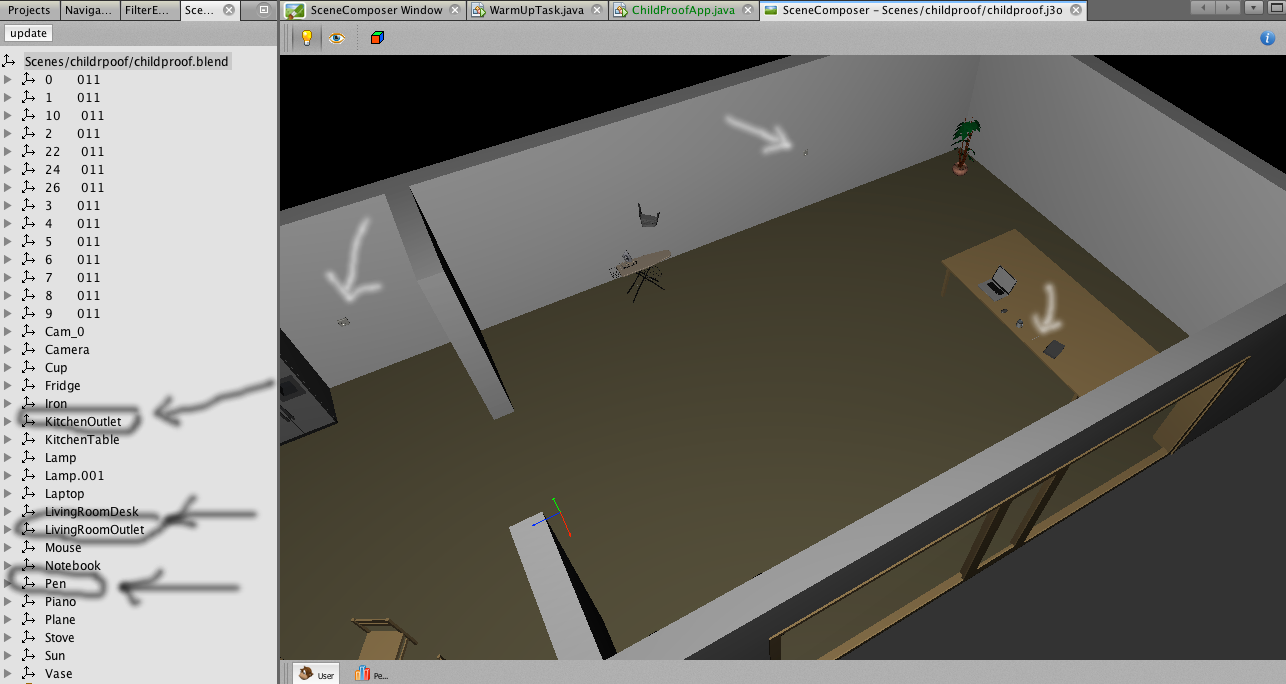
\includegraphics[width=\linewidth]{gfx/Chapter_SD_UserGuide/objects_to_identify}
	\caption{Example objects to identify in the Scene Composer}
	\label{fig:sd_objects_to_identify}
\end{figure}

Identify the objects in the ''SceneExplorer Window'' on the left or by RIGHT-CLICKing on them in the ''SceneComposer''. Either way, as you identify them, they get highlighted in the ''SceneComposer'' on the right, as depicted in Figure \ref{fig:sd_scene_composer}.
\begin{figure}[H]
	\centering
	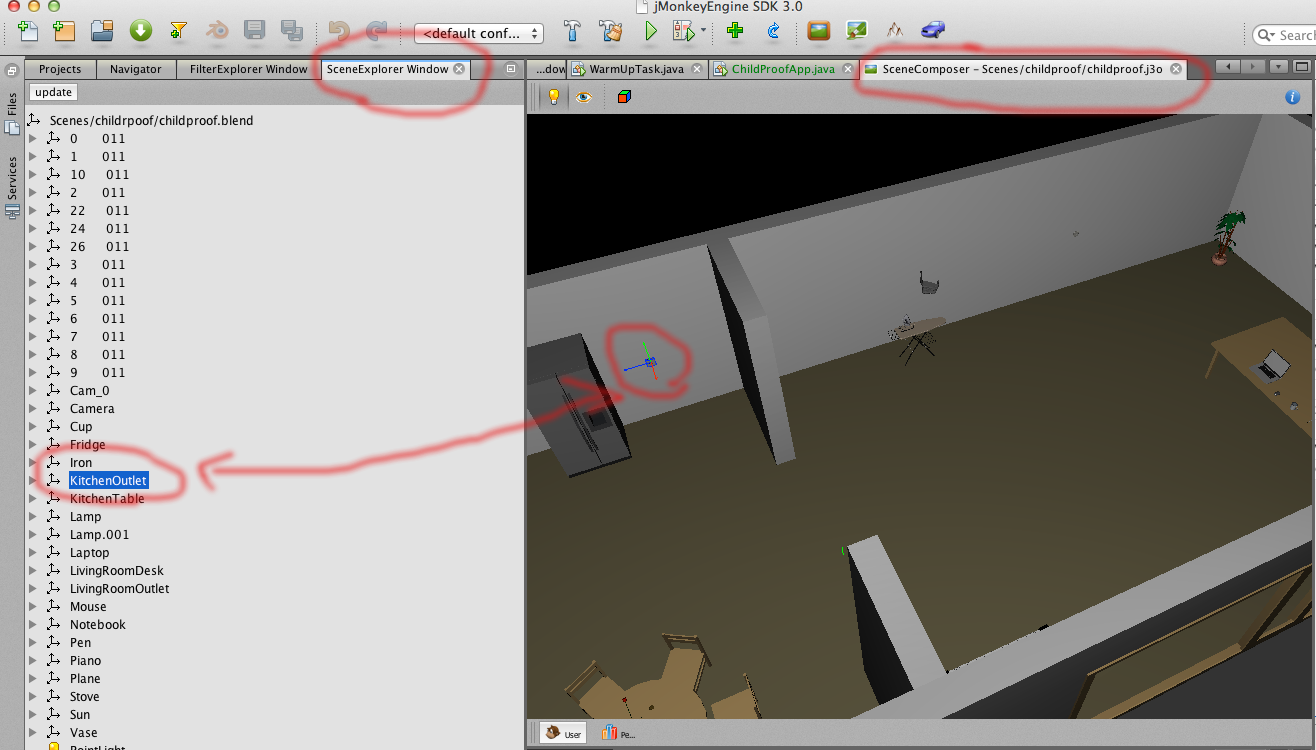
\includegraphics[width=\linewidth]{gfx/Chapter_SD_UserGuide/scenecomposer}
	\caption{Scene Composer}
	\label{fig:sd_scene_composer}
\end{figure}

To augment the objects with context data:
\begin{enumerate}
	\item Right click the object in the ''SceneComposer Window'' and select the ''Add User Data'' as illustrated in Figure \ref{fig:sd_add_user_data}.
		\begin{figure}[H]
			\centering
			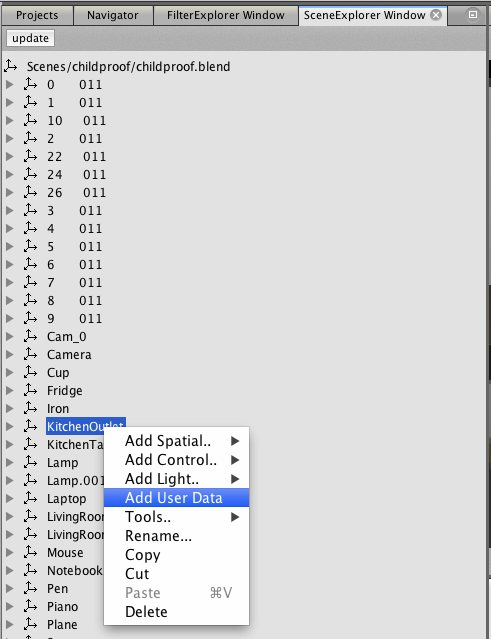
\includegraphics[width=0.8\linewidth]{gfx/Chapter_SD_UserGuide/add_user_data}
			\caption{Add User Data action}
			\label{fig:sd_add_user_data}
		\end{figure}

	\item In the name field enter enter EGOCENTRIC\_CONTEXT\_DATA. From the drop-down select ''Custom'' and choose ''dk.itu.bodysim. context.EgocentricContextData''. This will bring up the configuration form depicted in Figure \ref{fig:sd_config_form}.
		\begin{figure}[H]
			\centering
			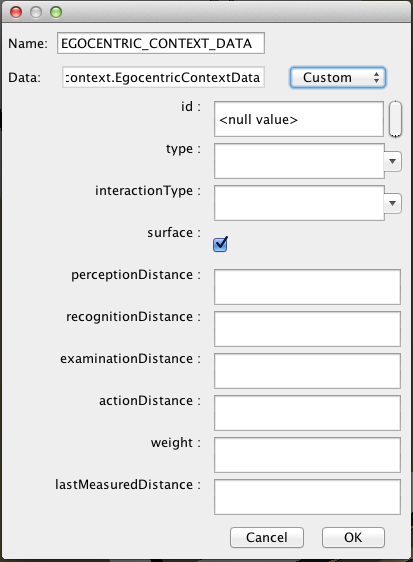
\includegraphics[width=0.8\linewidth]{gfx/Chapter_SD_UserGuide/ssmconfig}
			\caption{Ego Metadata Configuration Form}
			\label{fig:sd_config_form}
		\end{figure}

	\item Configure the ID with a unique name (e.g. KitchenOutlet for the outlet in the kitchen) and the ''interactionType'' with ''CUSTOM'' for Outlets (otherwise, the agent will be able to pick it up) and ''PICK\_UP'' for the Pen.

	\item The rest of the parameters will take meaningful default values. Although, to fine tune the classification, the option to configure them is there.

	\item Once done, hit the OK button.
\end{enumerate}

After you have configured all the objects you want to track, from the File menu select the ''Save All'' option.\\

You can close the SceneComposer now.\\
% section sd_identify_objects (end)